\documentclass[11pt]{scrartcl}
\usepackage[parfill]{parskip}
\usepackage{graphicx}
\usepackage{booktabs}
\usepackage{tabulary}
\usepackage{float}

\title{\textbf{Economic Aspects\\
                Lesson 4}}
\subtitle{Open Core Business Model}
\author{Jesús M. González-Barahona}
\date{\today}

\begin{document}

\maketitle

\section{OpenCore business model}

Questions about OpenCore business model.

\begin{itemize}

\item Choose a company that uses OpenCore business model and describe the main goals.

\par Rapid7\footnote{http://www.rapid7.com/} with Metasploit\footnote{http://www.metasploit.com/} - Licence 3-clause BSD\footnote{http://www.metasploit.com/license.jsp}.

\emph{The Metasploit Project develops the Metasploit Framework for penetration testing and includes an exploit database. The framework is used by network security professionals to perform penetration testing, system administrators to verify patch installations, product vendors to perform regression testing, and security researchers world-wide. Created by HD Moore, the Metasploit project was acquired by Rapid7 in October 2009.}

\par Has 4 Metasploit Frameworks

\begin{itemize}
    \item Framework
    \item Community
    \item Express
    \item Pro
\end{itemize}

\begin{figure}[H]
    \begin{center}
        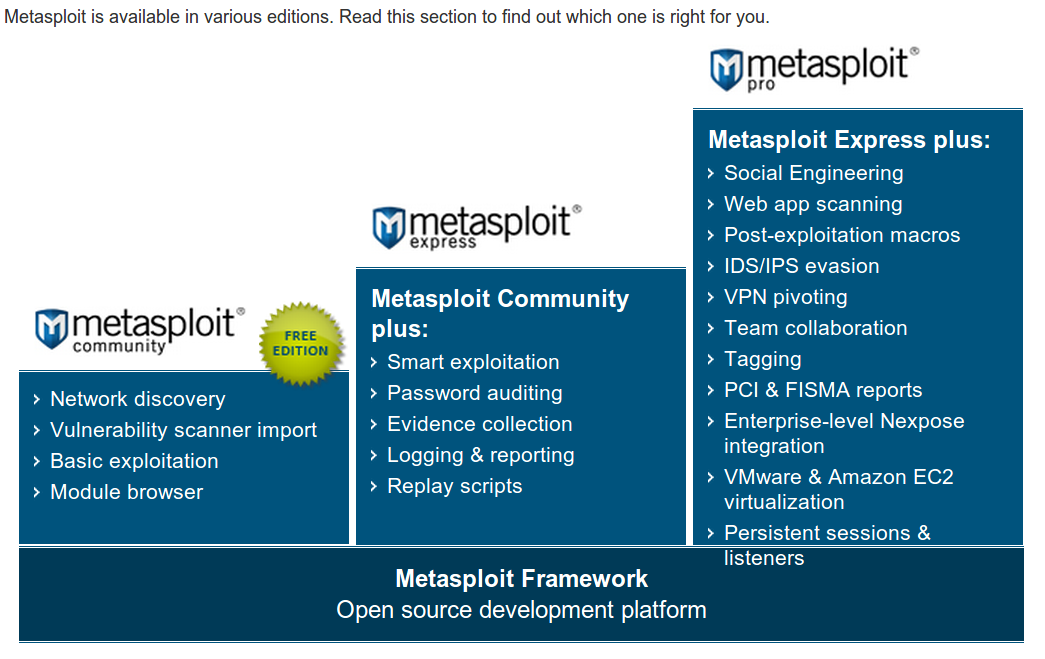
\includegraphics[width=0.9\textwidth]{images/metasploit-frameworks.png}
        \caption{Metasploit Frameworks}
        \label{fig:metasploit-fw}
    \end{center}
\end{figure}

Released into the Community Framework enhancements private products but after a while.

\item Is the company forced to follow this model or could afford to move to a free model (any we have seen)?

\begin{itemize}
    \item Product specialists for metasploit as expertise.
    \item Platform providers installing all you need to get a Security Suite.
    \item Legal certification/consulting, certification, menthoring, formation courses.
    \item Selection/consulting, Security consulting company.
\end{itemize}

\item Statement why OpenCore used, if any.

\par Metasploit is a security product that Rapid7 obtained from the purchase of the company and the community maintains that houses around it. So you must keep in mind the FLOSS-oriented model.

\par Also shown in figures growth in Community product development:

\emph{6 releases in the first 12 months after our acquisition Compared to one release in the 18 months prior.}

\par The Metasploit community has grown around 25,000 users in 2009 to 125,000 in 2012 after buying the company. These are some very good numbers.

\par They use the private model to continue maintaining the free versions for the community.

\par They have an Open Source commitment\footnote{http://www.metasploit.com/about/open-source/} in which is included its aim to improve Open Source in distinct ways:

    \begin{itemize}
        \item Donate money to other FLOSS projects.
        \item Free source code from private versions to community versions.
    \end{itemize}

\item Feedback to the particular case and in general on the model OpenCore, business, community, learning.

\begin{itemize}
    \item Facilitates the use of the tool to a greater number of users by the security measures.
    \item Commitment to the community.
\end{itemize}

\par In general aspects; OpenCore incentives the community to create solutions derived from base product, the innovation comes from the community. If there is a need in the community, that it will find the solution to the need may be better than the private solution. By creating a community around the product better and more knowledgeable.

\par The pattern moves across a time window, ie not seem feasible OpenCore lifetime tends to complete release code. If the product is successful, it is much easier to occur. So if the company knows evolve within the same model can feed knowledge with the community, generating every 'x' time new private solutions but in turn, have been clear that releasing them after a while.

\end{itemize}

\end{document}
